\chapter{Tkinter概述}
\section{Tkinter简介}
Tkinter是Python的标准GUI（图形用户界面）工具包，它是Python的一个内置模块，用于创建GUI应用程序。Tkinter是一个跨平台的工具包，它可以在Windows、Mac OS X和Linux等操作系统上运行。



\section{标准属性}
标准属性也就是所有控件的共同属性，如大小，字体和颜色等等。
\begin{table}[]
    \begin{tabular}{|l|l|}
    \hline
    \multicolumn{1}{|c|}{\textbf{属性}} & \multicolumn{1}{c|}{\textbf{描述}} \\ \hline
    Dimensions                          & 控件的高度和宽度。                     \\ \hline
    Colors                              & 控件的前景和背景颜色。                   \\ \hline
    Fonts                               & 控件的字体。                        \\ \hline
    Anchor                              & 控件的对齐方式。                      \\ \hline
    Relief                              & 控件的边框样式。                      \\ \hline
    Bitmaps                             & 控件的位图。                        \\ \hline
    Cursors                             & 控件的光标样式。                      \\ \hline
    \end{tabular}
    \caption{标准属性}
\end{table}

\section{tkinter的坐标系与颜色格式}
\subsection{坐标系}
Tkinter的坐标系是以窗口的左上角为原点，向右为x轴正方向，向下为y轴正方向。
\begin{figure}[htpb]
    \centering
    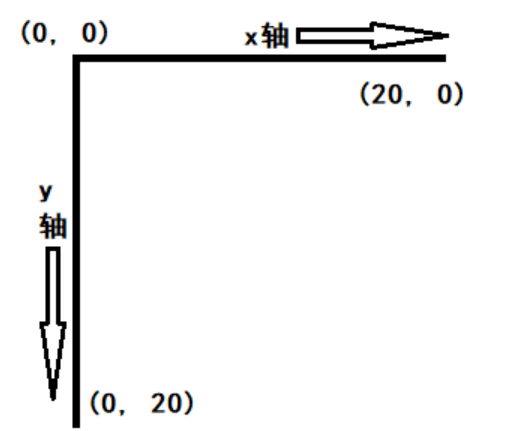
\includegraphics[width=0.6\textwidth]{part/图形化/pic/Tkinter/概述/tkinter坐标系.png}
    \caption{Tkinter坐标系}
    \label{fig:tkinter坐标系}
\end{figure}

如图\ref{fig:tkinter坐标系}所示，窗口的左上角坐标为(0,0)，向右移动一个单位，坐标变为(1,0)，向下移动一个单位，坐标变为(0,1)。

其中1个单位的长度为1个像素。

\subsection{颜色格式}
当在tkinter中设置颜色时，可以用两种表示颜色的方式
\begin{enumerate}[label=\arabic*)]
    \item 十六进制表示法：
    
    \codeinline{\#RRGGBB}，其中RR代表红色的十六进制值，GG代表绿色的十六进制值，BB代表蓝色的十六进制值。
    \item 颜色名：
    
    可以使用颜色名，如'\codeinline{red}'代表红色，'\codeinline{blue}'代表蓝色。
\end{enumerate}


\section{根窗口}
在Tkinter中，每个控件都是一个独立的对象，这些控件都是以根窗口为基础的。
根窗口是所有控件的父窗口，所有的控件都是根窗口的子控件。
\begin{lstlisting}[style=demostyle,numbers=none]
from tkinter import *

# screenName: 屏幕名字
# baseName: 基本名字
# className: 类名
# useTk: 是否使用Tk
# sync: 是否同步
# use: 使用
root = Tk(screenName=None, baseName=None, className='Tk', useTk=1, sync=0, use=None)
\end{lstlisting}

\begin{lstlisting}[style=pythonstyle,numbers=left]
from tkinter import *
 
root = Tk()
mainloop() # 循环显示这个窗口

# 也可以用
# while True:
#     if not root.update():
#         break
\end{lstlisting}

\subsection{根窗口的方法}
但是在实际编程中，我们通常不会使用这些参数，直接使用\codeinline{Tk()}即可，如果需要设置这些参数，可以在创建根窗口后再设置。
\begin{enumerate}[label=\arabic*)]
    \item \codeinline{title(string=None)}:	设置窗口的标题，同时返回窗口标题
    \item \codeinline{geometry(newGeometry=None)}:	设置窗口的尺寸大小，同时返回当前窗口尺寸
    \item \codeinline{iconbitmap(bitmap=None)}:	设置窗口的图标，需指定图标文件(*.ico)的位置
    \item \codeinline{resizable(width=None, height=None)}:	设定是否能够改变窗口的宽和高尺寸
    \item \codeinline{destroy()}:	销毁窗口，也就是把窗口关掉
    \item \codeinline{config(**kw)}:	设置窗口的属性，如背景色、前景色、字体、大小等}
\end{enumerate}

\begin{lstlisting}[style=pythonstyle,numbers=left]
from tkinter import *
 
root = Tk()
root.title('窗口标题')      # 设置窗口标题
#root.geometry('300x300')   # 设置窗口尺寸
root.geometry("300x100+20+50") # 设置窗口尺寸为300x100，位于与屏幕最左边相隔20像素，与屏幕最上方相隔50像素
root.iconbitmap('favicon.ico') # 设置窗口图标
root.resizable(width=False, height=True) # 设置窗口的宽度和高度是否可以改变
# root.destroy() # 销毁窗口

mainloop()
\end{lstlisting}

运行结果如图\ref{fig:根窗口设置方法}所示。
\begin{figure}[htpb]
    \centering
    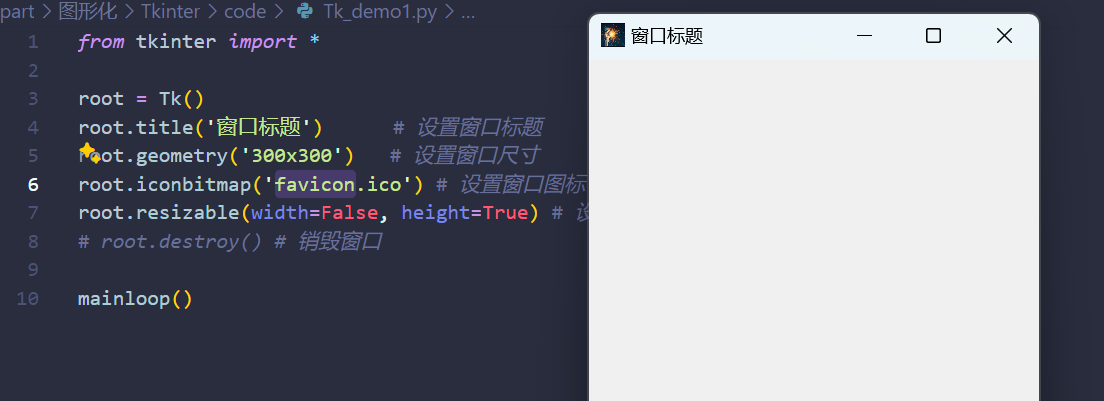
\includegraphics[width=0.6\textwidth]{part/图形化/pic/Tkinter/概述/根窗口设置方法.png}
    \caption{根窗口设置方法}
    \label{fig:根窗口设置方法}
\end{figure}

\section{Tkinter 组件}
tkinter支持很多组件（又叫控件、小部件等等），可以帮助你完成一些功能。组件根据坐标被排列在容器(container)中，窗口的界面是该窗口中最大的容器。

\begin{table}[]
    \begin{tabular}{|l|l|}
    \hline
    \multicolumn{1}{|c|}{\textbf{控件}} & \multicolumn{1}{c|}{\textbf{描述}}       \\ \hline
    Button                              & 按钮控件；在程序中显示按钮。                         \\ \hline
    Canvas                              & 画布控件；显示图形元素如线条或文本                      \\ \hline
    Checkbutton                         & 多选框控件；用于在程序中提供多项选择框                    \\ \hline
    Entry                               & 输入控件；用于显示简单的文本内容                       \\ \hline
    Frame                               & 框架控件；在屏幕上显示一个矩形区域，多用来作为容器              \\ \hline
    Label                               & 标签控件；可以显示文本和位图                         \\ \hline
    Listbox                             & 列表框控件；在Listbox窗口小部件是用来显示一个字符串列表给用户     \\ \hline
    Menubutton                          & 菜单按钮控件，用于显示菜单项。                        \\ \hline
    Menu                                & 菜单控件；显示菜单栏,下拉菜单和弹出菜单                   \\ \hline
    Message                             & 消息控件；用来显示多行文本，与label比较类似               \\ \hline
    Radiobutton                         & 单选按钮控件；显示一个单选的按钮状态                     \\ \hline
    Scale                               & 范围控件；显示一个数值刻度，为输出限定范围的数字区间             \\ \hline
    Scrollbar                           & 滚动条控件，当内容超过可视化区域时使用，如列表框。.             \\ \hline
    Text                                & 文本控件；用于显示多行文本                          \\ \hline
    Toplevel                            & 容器控件；用来提供一个单独的对话框，和Frame比较类似           \\ \hline
    Spinbox                             & 输入控件；与Entry类似，但是可以指定输入范围值              \\ \hline
    PanedWindow                         & PanedWindow是一个窗口布局管理的插件，可以包含一个或者多个子控件。 \\ \hline
    LabelFrame                          & labelframe 是一个简单的容器控件。常用于复杂的窗口布局。      \\ \hline
    tkMessageBox                        & 用于显示你应用程序的消息框。                         \\ \hline
    \end{tabular}
    \caption{Tkinter控件}   
\end{table}

\subsection{Label 标签}
\begin{lstlisting}[style=demostyle,numbers=none]
# text	显示的文本
# font	文本的字体
# image	显示的图片
# bitmap	显示的位图，和image只能指定一个
# textvariable	绑定的文本变量
# compound	当文本和图片同时显示时，图片位于文本的方位，可以是top, bottom, left, right, center，如：设置为top表示图片位于文本上方
# padx	标签内容与左右的间距
# pady	标签内容与上下的间距
# anchor	文本靠标签哪个方向显示，可以是n,s,w,e,ne,nw,sw,se,center，即北、南、西、东、东北、西北、西南、东南、中间，默认靠中间显示
# justify	文本的对齐方式，可以是left, right, center，默认是center
# wraplength	自动换行字符数量，到达数量后文本会自动换一行显示
# relief	标签的边框样式，可以是flat, raised, sunken, groove, ridge，默认是flat

Label(master=None, cnf={}, **kw)
\end{lstlisting}

\subsection{Button 按钮}
Button即按钮，可以绑定一个回调函数，用户点击时将会执行这个函数。
\begin{lstlisting}[style=demostyle,numbers=none]
# text	显示的文本
# font	文本的字体
# image	显示的图片
# bitmap	显示的位图，和image只能指定一个
# textvariable	绑定的文本变量
# compound	当文本和图片同时显示时，图片位于文本的方位，可以是top, bottom, left, right, center，如：设置为top表示图片位于文本上方

Button(master=None, cnf={}, **kw)
\end{lstlisting}

\begin{lstlisting}[style=pythonstyle,numbers=left]
from tkinter import *
 
root = Tk()
 
def callback():
    print("你点了一下按钮")
 
button = Button(root, text="按钮", command=callback)
button.pack()
 
mainloop()
\end{lstlisting}

\begin{figure}[htpb]
    \centering
    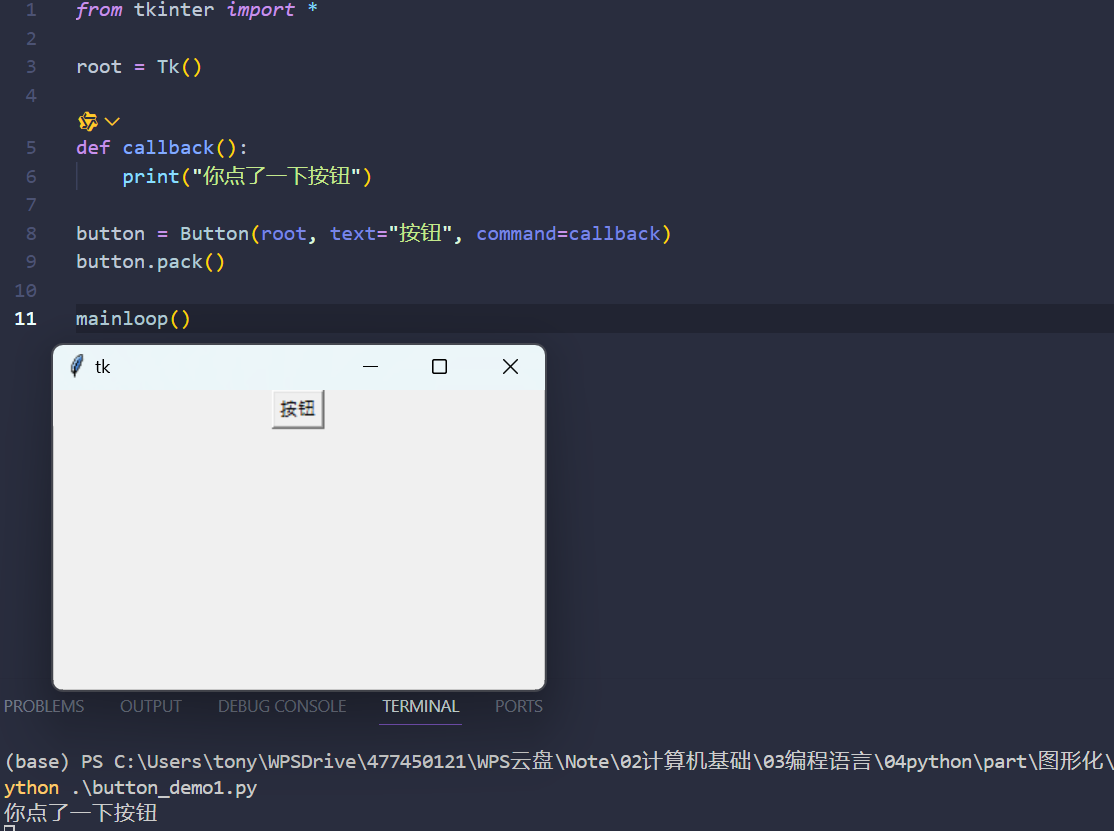
\includegraphics[width=0.6\textwidth]{part/图形化/pic/Tkinter/概述/button绑定事件.png}
    \caption{button绑定事件}
    \label{fig:button绑定事件}
\end{figure}

\subsubsection{activeforeground和activebackground 按键背景颜色}

如果鼠标长按按钮，那么按钮不会被触发，而是松开鼠标后触发。这时候，按钮处于一种激活状态。我们可以设置激活时按钮的前景和背景颜色：
\begin{lstlisting}[style=pythonstyle,numbers=left]
from tkinter import *
 
root = Tk()
 
def callback():
    print("你点了一下按钮")
 
button = Button(root, text="按钮", command=callback, activeforeground="red", activebackground="yellow")
button.pack()
 
mainloop()
\end{lstlisting}

\section{布局管理}
组件需要在创建后，摆放到屏幕上。一共有三种摆放的方式：
\begin{enumerate}[label=\arabic*)]
    \item \codeinline{pack}：组件会自动填充整个容器，组件之间会自动排列。
    \item \codeinline{grid}：组件会自动填充整个容器，组件之间会自动排列。
    \item \codeinline{place}：组件会根据指定的位置摆放。
\end{enumerate}

\textcolor{red}{\textbf{在同一个容器中，只能使用一种布局方式}}

\subsection{pack 简单的布局}
\begin{enumerate}[label=\arabic*)]
    \item \codeinline{side}: 组件靠哪个方向排放，可以是\codeinline{top}, \codeinline{bottom}, \codeinline{left}, \codeinline{right}, \codeinline{center}，默认是top。
    \item \codeinline{fill}: 组件的填充方式，可以是none, x, y, both，默认是none。
    \begin{enumerate}[itemindent=1em,label=\arabic*)]
        \item \codeinline{none}: 不填充
        \item \codeinline{x}: 横向填充
        \item \codeinline{y}: 纵向填充
        \item \codeinline{both}: 横向纵向填充
    \end{enumerate}
    \begin{figure}[htpb]
        \centering
        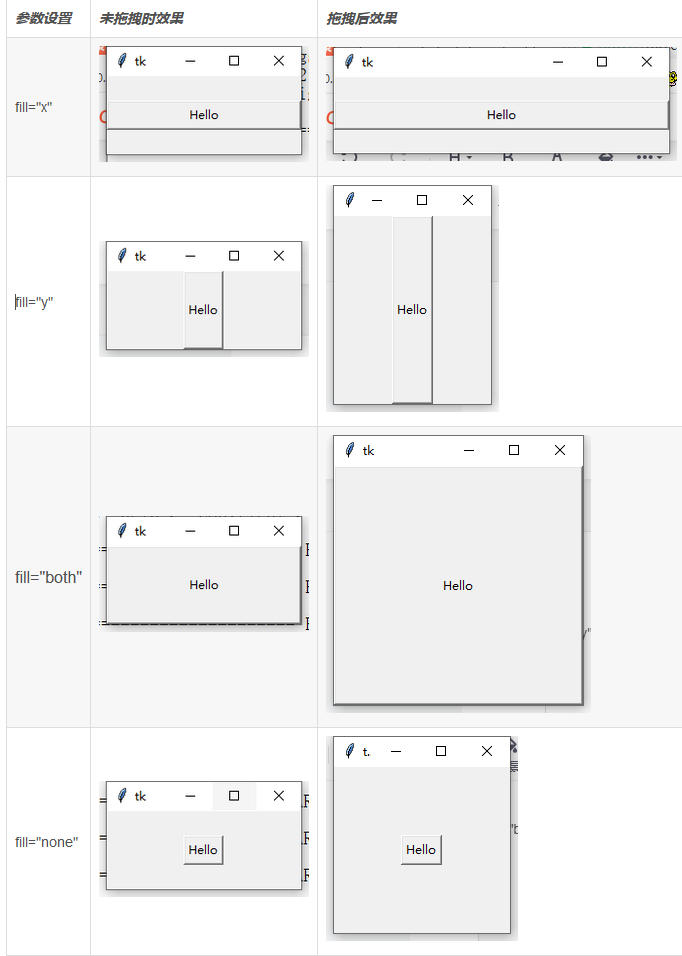
\includegraphics[width=0.4\textwidth]{part/图形化/pic/Tkinter/概述/pack-fill效果.png}
        \caption{fill效果}
    \end{figure}
    
    \item \codeinline{expand}: 组件是否自动扩展,如设置为True，当窗口中有别的可用空间时，将会自动把组件居中摆放，并且拖拽后仍然适应窗口大小。默认为False。，默认是false。

\begin{lstlisting}[style=pythonstyle,numbers=left]
from tkinter import *
 
root = Tk()
root.geometry("200x80")
 
w1 = Button(root, text="W1")
w1.pack(expand=True)
 
w2 = Button(root, text="W2")
w2.pack(expand=True)
 
root.mainloop()
\end{lstlisting}
\begin{figure}[htpb]
    \centering
    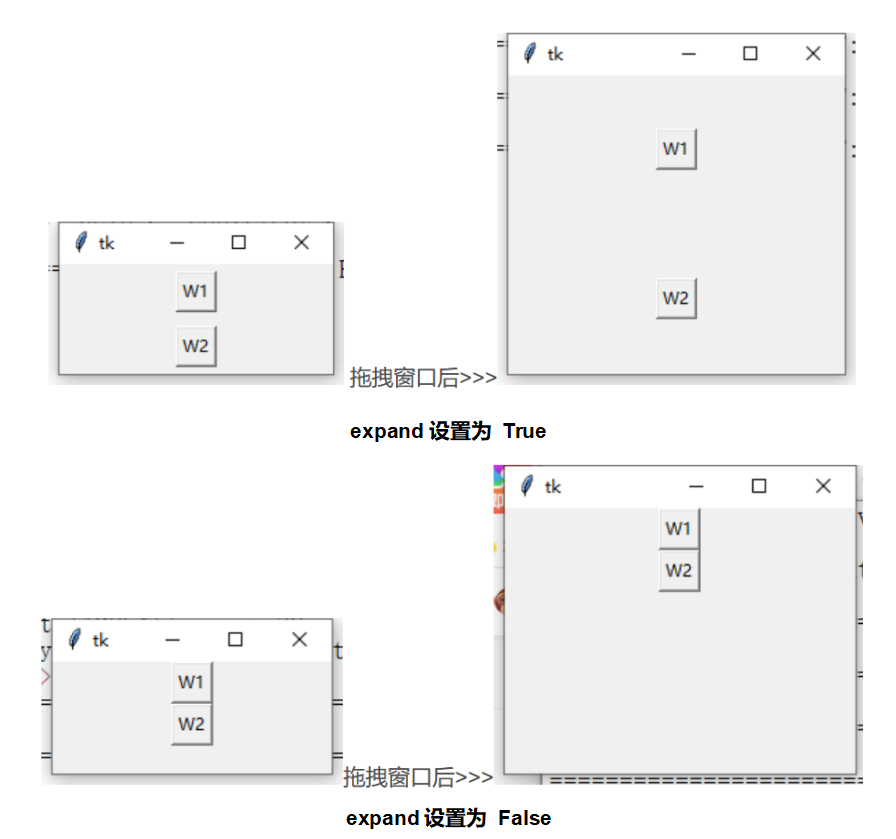
\includegraphics[width=0.6\textwidth]{part/图形化/pic/Tkinter/概述/pack-expand效果.png}
    \caption{expand效果}
\end{figure}
    \item \codeinline{padx}: 组件的水平间距，默认是0。
    \item \codeinline{pady}: 组件的垂直间距，默认是0 
\begin{lstlisting}[style=pythonstyle,numbers=left]
from tkinter import *
 
root = Tk()
 
w1 = Button(root, text="Hello")
w1.pack(padx=50, pady=30) #左右间隔50，上下间隔30
 
root.mainloop()
\end{lstlisting}

\begin{lstlisting}[style=pythonstyle,numbers=left]
from tkinter import *
 
root = Tk()
 
w1 = Button(root, text="Hello")
w1.pack(padx=(50, 40), pady=(30, 60)) #左间隔50，右间隔40，上间隔30，下间隔60
 
root.mainloop()
\end{lstlisting}

    \begin{figure}[htpb]
        \centering
        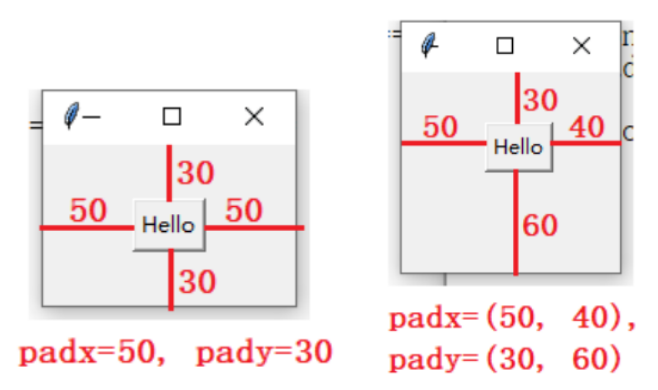
\includegraphics[width=0.6\textwidth]{part/图形化/pic/Tkinter/概述/pack-padx和pady的效果.png}
        \caption{padx和pady的效果}
    \end{figure}


    \item \codeinline{ipadx}: 表示内部与组件边框的间隔的水平间距，默认是0。  
    \item \codeinline{ipady}: 表示内部与组件边框的间隔的垂直间距，默认是0 
\begin{lstlisting}[style=pythonstyle,numbers=left]
from tkinter import *
    
root = Tk()
root.geometry("400x200")
    
w1 = Button(root, text="Hello")
w1.pack(ipadx=40, ipady=40)
    
root.mainloop()
\end{lstlisting}
    \begin{figure}[htpb]
        \centering
        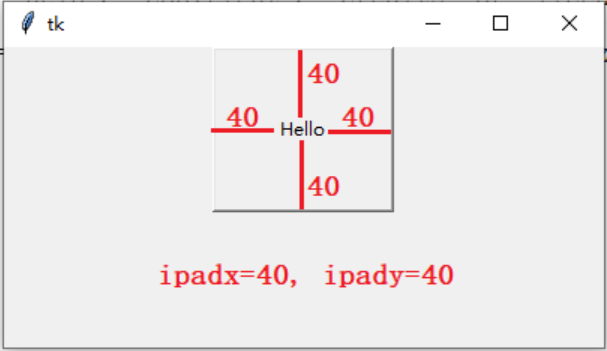
\includegraphics[width=0.4\textwidth]{part/图形化/pic/Tkinter/概述/pack-ipadx和ipady的效果.png}
        \caption{ipadx和ipady的效果}
    \end{figure}
    

    \item \codeinline{anchor}: 当排放组件的可用空间要多于所需空间时，组件靠哪个方向排放，可选项是八个方位和中心\codeinline{n},\codeinline{s},\codeinline{w},\codeinline{e},\codeinline{ne},\codeinline{nw},\codeinline{sw},\codeinline{se},\codeinline{center}，默认是center。

\begin{lstlisting}[style=pythonstyle,numbers=left]
from tkinter import *
    
root = Tk()
root.geometry("200x200")
    
w1 = Button(root, text="多余空间靠左")
w1.pack(anchor="w")
    
root.mainloop()
\end{lstlisting}
\begin{figure}[htpb]
    \centering
    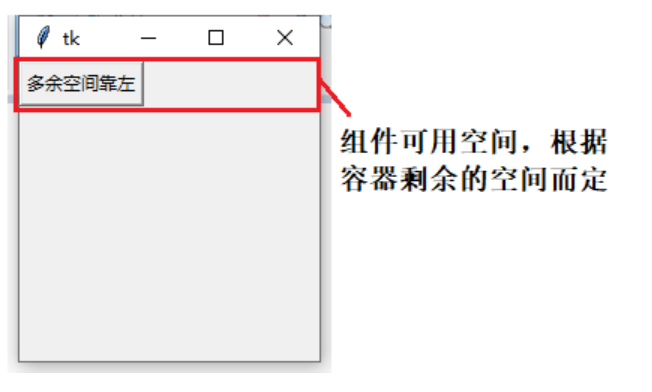
\includegraphics[width=0.6\textwidth]{part/图形化/pic/Tkinter/概述/anchor多余空间.png}
    \caption{anchor多余空间}
\end{figure}

\end{enumerate}

\subsection{grid 网格宫布局}

pack布局方式适合于简单的布局，在同一容器内，只能进行上下左右四方向的布局。而grid可以实现网格布局，根据行和列指定组件的位置。grid布局和pack一样都支持padx, pady, ipadx, ipady这几个参数。

\begin{enumerate}[label=\arabic*)]
    \item \codeinline{row}: 组件所在行的索引，从0开始,第一行就是\codeinline{row=0}。
    \item \codeinline{column}: 组件所在列的索引，从0开始。

\begin{lstlisting}[style=pythonstyle,numbers=left]
from tkinter import *
 
root = Tk()
root.geometry("400x200")
 
Button(root, text="0行0列").grid(row=0, column=0)
Button(root, text="1行0列").grid(row=1, column=0)
Button(root, text="0行1列").grid(row=0, column=1)
Button(root, text="1行1列").grid(row=1, column=1)
 
root.mainloop()
\end{lstlisting}

\begin{figure}[htpb]
    \centering
    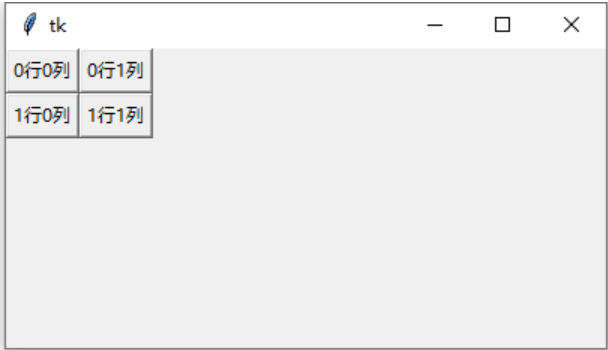
\includegraphics[width=0.6\textwidth]{part/图形化/pic/Tkinter/概述/grad-column和row效果.png}
    \caption{column和row的效果}
\end{figure}
    \item \codeinline{rowspan}: 组件占用的行数，默认是1。
    \item \codeinline{columnspan}: 组件占用的列数，默认是1。

\begin{lstlisting}[style=pythonstyle,numbers=left]
from tkinter import *
 
root = Tk()
root.geometry("400x200")
 
Button(root, text="0行0列").grid(row=0, column=0)
Button(root, text="1行0列").grid(row=1, column=0)
Button(root, text="0行1列(占两行)").grid(row=0, column=1, rowspan=2)
 
root.mainloop()
\end{lstlisting}

\begin{lstlisting}[style=pythonstyle,numbers=left]
from tkinter import *
 
root = Tk()
root.geometry("400x200")
 
Button(root, text="0行0列").grid(row=0, column=0)
Button(root, text="0行1列").grid(row=0, column=1)
Button(root, text="1行0列(占两列)").grid(row=1, column=0, columnspan=2)
 
root.mainloop()
\end{lstlisting}
    \begin{figure}[htpb]
        \centering
        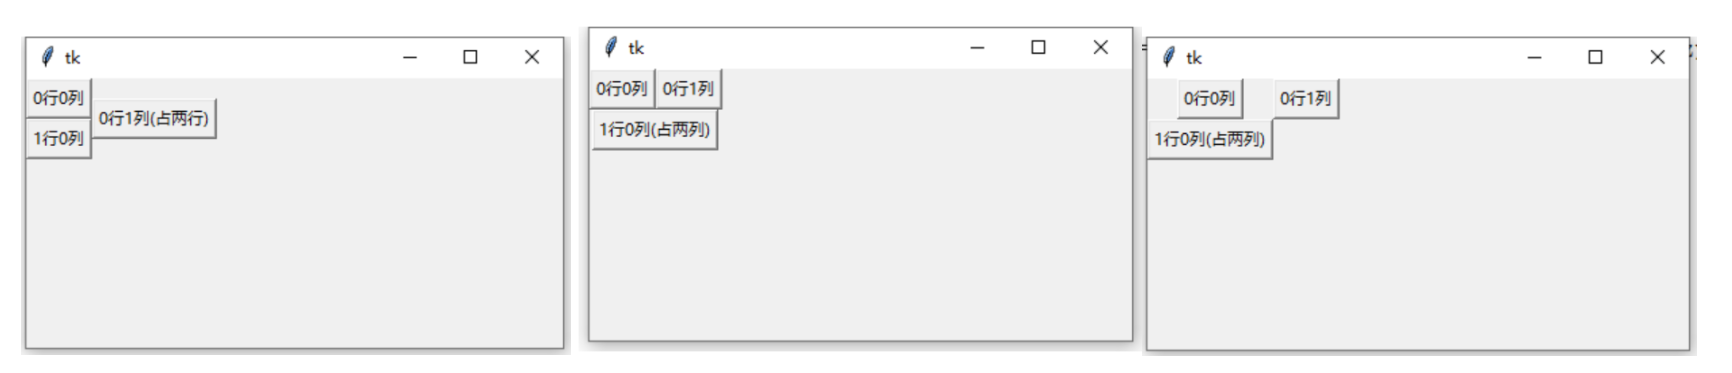
\includegraphics[width=0.8\textwidth]{part/图形化/pic/Tkinter/概述/grad-columnspan和rowspan效果.png}
        \caption{columnspan和rowspan的效果}
    \end{figure}


    \item \codeinline{sticky}: 组件的摆放位置(在pack布局中和anchor类似，表示组件的方位，同时也可以达到fill的功能)，可以是\codeinline{n},\codeinline{s},\codeinline{w},\codeinline{e},\codeinline{ne},\codeinline{nw},\codeinline{sw},\codeinline{se}，默认是\codeinline{n}。

    \begin{enumerate}[label=\arabic*)]
        \item \codeinline{n}: 组件在顶部。
        \item \codeinline{s}: 组件在底部。
        \item \codeinline{w}: 组件在左侧。
        \item \codeinline{e}: 组件在右侧。
        \item \codeinline{ne}: 组件在右上角。
        \item \codeinline{nw}: 组件在左上角。
        \item \codeinline{sw}: 组件在左下角。
        \item \codeinline{se}: 组件在右下角。
        \item \codeinline{center}: 组件在容器的中心。
        \item \codeinline{ns}: 组件在顶部和底部。
        \item \codeinline{ew}: 组件在左侧和右侧。
        \item \codeinline{nesw}: 组件在左上角、右上角、右下角、左下角。
    \end{enumerate}

    \begin{figure}[htpb]
        \centering
        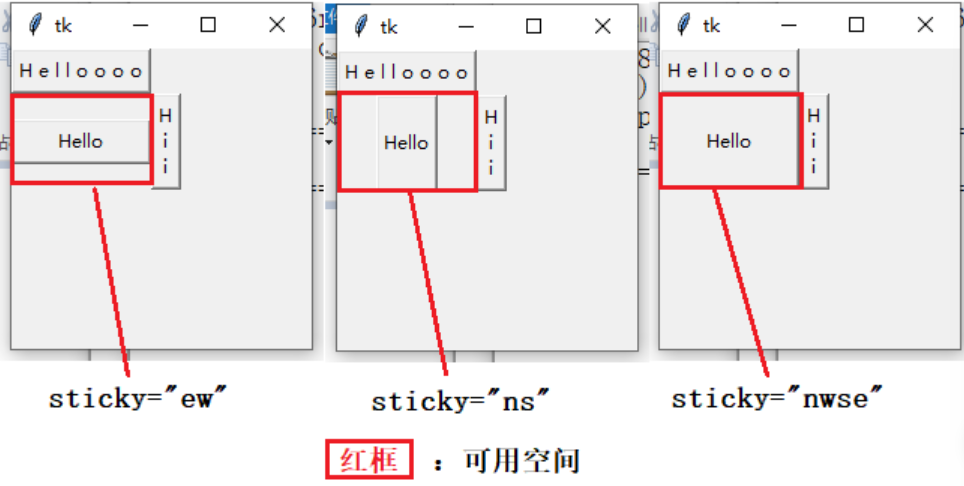
\includegraphics[width=0.6\textwidth]{part/图形化/pic/Tkinter/概述/grad-sticky效果.png}
        \caption{caption}
        \label{fig:label}
    \end{figure}
    
    
\end{enumerate}

\subsection{place 布局}
place布局适用于更加复杂的，需要准确摆放组件的容器。这种布局不是很常用，因为使用比较麻烦，需要提供xy坐标以及组件的width和height（以像素为单位），place布局不支持padx……几个参数。

\begin{enumerate}[label=\arabic*)]
    \item \codeinline{x}和\codeinline{y}：组件在x轴和y轴上的位置，单位为像素。
    \item \codeinline{anchor}：组件的锚选项，可选有八个方位，以及center。
    
    意思是：组件anchor位置的坐标设置为x,y。
    
    如：anchor="n"的时候，如果x=100, y=100，那么组件的最上面的中间的那个点的位置就是(100, 100)。

    \item \codeinline{width}和\codeinline{height}：指定组件排放时的宽和高。
    \item \codeinline{relx}和\codeinline{rely}：组件在x轴或y轴相对于整个容器的位置，是一个0-1之间的浮点数，表示组件位于整个容器的位置。比如想要把组件的x设在容器30%的位置，则可以把位置设为0.3.如果想要把组件居中，就设置relx=0.5, rely=0.5, anchor="center"。
    \item \codeinline{relwidth}和\codeinline{relheight}：指定组件相对于容器的宽与高，是一个0-1之间的浮点数。组件宽是容器宽的50\%，则可以把relwidth设置为0.5.
\end{enumerate}



\section{Tkinter的事件处理}


